\documentclass[11pt]{article}

\usepackage{listings}
\usepackage[utf8]{inputenc}
\usepackage[T1]{fontenc}
\usepackage[french]{babel}
\usepackage{fixltx2e}
\usepackage{graphicx}
\usepackage{longtable}
\usepackage{float}
\usepackage{wrapfig}
\usepackage{soul}
\usepackage{textcomp}
\usepackage{marvosym}
\usepackage{wasysym}
\usepackage{latexsym}
\usepackage{amssymb}
\usepackage{hyperref}

\hypersetup{
  colorlinks=true,
}

\usepackage{glossaries}

%%glossary entries

\newglossaryentry{tachePrincipale}
{
  name=tâche principale,
  description={Une tâche n'ayant aucune tâche mère}
}

\newglossaryentry{soustache}
{
  name=sous-tâche,
  description={Une tâche liée à une tâche mère. Une relation de
    dépendance existe. Notamment, si une tâche mère est supprimée,
    toutes ses tâches filles (ses sous-tâches), sont supprimées}
}

\newglossaryentry{technocentre}
{
  name=technocentré,
  description={Se dit d'une interface basée sur la technologie. On se
  sert des capacités connues d'une machine pour construire une interface à
  l'image de la machine}
}

\newglossaryentry{anthropocentre}
{
  name=anthropocentré,
  description={Se dit d'une interface basée sur l'humain. On se sert
    des repères culturels pour construire une interface à l'image de l'homme}
}

\newglossaryentry{metaphore}
{
  name=métaphore,
  description={Terme utilisé pour décrire un type d'interface
    particulier. La métaphore de l'arbre est une interface proposant
    une vue de type arbre ie chaque élement peut être parent d'un
    autre élément du même type. Ici, une tâche peut être mère d'une
    autre tâche. La seconde dépend alors de la première}
}

\makeglossaries

\author{Grégoire Jadi \and{} Rémi Bois \and{} Loïc Jankowiak}
\title{TASER \\
Gestionnaire Avancé de Tâches}

\begin{document}

\maketitle
\begin{figure}[h]
  \centering
  
\includegraphics{img/logo_nantes.png}  
\end{figure}

\newpage
\tableofcontents
\newpage


\section{Présentation}

L'objectif de ce projet était de mettre en pratique les différentes
techniques permettant de réaliser des interfaces graphiques.

Nous devions donc définir et concevoir une interface homme machine
(IHM), réalisée à l'aide du framework graphique Qt, servant à la
gestion avancée de tâches. L'utilisateur devait entre autre pouvoir
\begin{itemize}
\item ordonner des tâches;
\item fixer une date aux tâches;
\item gérer des templates de tâches;
\end{itemize}
On se référera au sujet pour une liste exhaustive des fonctionalités
attendues.

Nous allons maintenant présenter notre implémentation,
TASER\footnote{TASk managER}, détailler et expliquer les différents
choix d'interface et d'ergonomie qui ont été fait.


\section{Les premières idées}

Une fois que nous avons pris connaissance du sujet, nous nous sommes
mis d'accord pour chacun réfléchir de notre côté pendant une semaine
sur le sujet et ainsi nous retrouver avec chacun une proposition
d'interface non biaisée.

La confrontation des idées fut très intéressante car, comme nous
allons le voir, nous avons tous présenté une interface différente qui
présentent toutes des caractéristiques distinctes.

% TODO rajouter les premiers dessins + mini scénario de chaque interface
% TODO rajouter un tableau +/- pour chaque interface


\subsection{Une interface sobre}

Comme on peut le constater, la première interface est relativement
sobre.

L'utilisation de deux cadres est intéressante mais c'est une
organisation de l'espace de travail qui amènerait à montrer trop
d'informations à la fois.

De plus, c'est une interface qui rappelle beaucoup les grosses
applications dédiées à un domaine, elle est très «
\glslink{technocentre}{technocentrée}». 

La working copy de cette interface est disponible en annexe
\ref{ann:props} page \pageref{fig:sobre}.


\subsection{Une interface connue}

Cette deuxième interface utilise donc une vue arborescente des tâches
qui possède l'avantage d'être connue. En effet, la \gls{metaphore} de
l'arbre est déjà largement utilisée par les explorateurs de fichiers.
C'est pourquoi la réutilisation de ce design permet à l'utilisateur
d'être en terrain connu.

Cependant, bien que cette disposition soit plus légère que celle de
l'interface précédente, l'arbre reste assez lourd visuellement.

La working copy de cette interface est disponible en annexe \ref{ann:props} page \pageref{fig:connue}.


\subsection{Une interface sexy}

La dernière interface est fortement inspirée d'Org Mode, un mode
d'Emacs\footnote{Emacs est un excellent système d'exploitation à qui
  il ne manque qu'un éditeur de texte.} qui permet entre autre de
gérer des tâches.

Cette configuration est assez proche de la précédente, car elle
conserve l'idée d'organiser les tâches sous forme d'arbres. Elle nous
a semblé être celle se rapprochant le plus d'une idée intuitive la
représentation de tâches et de \gls{soustache}. Nous l'avons
considérée \glslink{anthropocentre}{anthropocentrée}.

De plus, comme l'un d'entre nous utilise beaucoup Org Mode, nous
savions que c'était une interface qui était utilisable.

Enfin, cette interface nous a semblé agréable à utiliser. Elle
ressemble aux interfaces des smartphones, utilisées dans un contexte
de détente. Les autres interfaces nous faisant penser davantage à des
logiciels de travail, nous étions satisfaits de cette différence et
souhaitions insister sur cet aspect. Nous avons jugé que notre
application serait destinée à être utilisée régulièrement, au
démarrage de l'ordinateur par exemple, pour vérifier si des choses
urgentes sont à faire, plutôt que comme outil branché en permanence et
monitorant le travail.

La working copy de cette interface est disponible en annexe \ref{ann:props} page \pageref{fig:sexy}.


\subsection{Bilan}

Il nous semble qu'avoir initialement réfléchi séparément fut une bonne
idée. Cela a permis à chacun de se faire sa propre idée de l'interface
qu'il désirait et d'avoir beaucoup d'idées différentes dès le départ.

De plus, comme nous avons fait le choix de la troisième interface assez
rapidement, nous étions relativement confiant dans notre choix,
puisque nous en avions déjà étudié deux autres.

Durant cette première étape nous avons donc décidé de la structure
générale de l'interface que nous souhaitions développer.

% TODO lien en annexes pour les storyboard/images restantes

\section{Un premier design}
\label{sec:premierDesign}

Une fois que nous avions l'idée globale de l'interface désirée. Nous
avons commencé à analyser plus en détail les différentes fonctions et
modes de fonctionnement de notre interface.


\subsection{Les fonctionnalités}

Nous avons commencé par lister l'ensemble des fonctionnalités que
notre interface graphique devait proposer ; il s'agit pour la plupart
de fonctionnalités classiques des gestionnaires de liste de tâches, à
savoir :
\begin{description}
\item[Ajouter/supprimer une tâche] Une tâche peut être ajoutée soit au
  niveau racine, soit en tant que sous-tâche d'une tâche existante. La
  suppression d'une tâche entraine automatiquement la suppression
  récursive de toutes ses sous-tâches. On trouvera une explication
  plus complète de la solution que nous avions initialement trouvée en
  section \ref{subsec:boutonFoison}.
\item[Valider une tâche] Principale fonctionnalité de l'application,
  elle permet de marquer une tâche comme ayant été effectuée ; une
  tâche peut également être invalidée.
\item[Déplier/replier une tâche] Un bouton permet d'afficher ou de
  masquer les sous-tâches d'une tâche, nous détaillons cette partie
  juste après loin dans la section \ref{sec:accordeon}. Au démarrage
  de l'application, seules les \glslink{tachePrincipale} sont
  visibles.
\item[Lier la date à la tâche parente] Chaque tâche possède une date
  limite (au-delà de laquelle elle est marquée comme en retard). Cette
  fonctionnalité permet, lorsque l'on décale une date de fin de tâche,
  de modifier automatiquement au besoin celles des sous-tâches liées.
\item[Monter/descendre une tâche] L'utilisateur peut réordonner à sa
  guise chacune des tâches et des sous-tâches de la liste.
\item[Liste ordonnée de sous-tâches] Afin de pouvoir satisfaire aux
  contraintes d'ordonnancement des tâches (par exemple, une tâche ne
  peut être validée que si une autre tâche a été validée
  précédemment), il est possible de définir chaque liste de tâches
  comme étant une liste ordonnée.

  Lorsqu'une liste de tâche est ordonnée, une tâche ne peut pas être
  validée tant que les tâches précédentes n'ont pas été validées. Dans
  le cas d'une liste non ordonnée, aucune contrainte n'est à respecter
  (il faut toutefois, pour cocher une tâche, que toutes ses
  sous-tâches soient validées).
\end{description}


% \begin{itemize}
% \item ajout, expand, order, close, update, check, link date, up\&down
% \item le "all one click"
% \item template via click droit
% \end{itemize}


\subsection{Le principe d'accordéon}
\label{sec:accordeon}

Nous souhaitions que notre interface permette l'affichage de
nombreuses tâches, sans pour autant perdre l'utilisateur dans trop de
données. Il nous fallait donc trouver une solution qui autoriserait
l'utilisateur d'afficher uniquement ce qu'il décide voir, tout en
laissant l'apparition de données supplémentaires à la portée d'un seul
clic. Le paradigme de l'accordéon, classique dans l'univers des
smartphones, nous a semblé être la solution adaptée.

Le paradigme de l'accordéon consiste à plier l'affichage : une tâche
contient toutes ses sous-tâches, et si l'on déplie une tâche, ses
sous-tâches s'affichent. Cet affichage est instinctif pour les
utilisateurs de smartphones et/ou de tablettes, friands de ce
paradigme.

Bien que fréquent sur les appareils mobiles, Qt ne propose pas de
Widget adoptant ce comportement. Nous nous sommes d'abord assurés que
simuler un tel comportement était possible via l'utilisation de layers
et de Widgets classiques. Ceci a été une réussite à l'exception du
fait qu'il nous a été impossible d'utiliser une animation.

Cependant, l'indentation des sous-tâches par rapport leur tâche mère
nous a semblée suffisante pour que l'utilisateur repère aisément
quelles tâches s'étaient dépliées, et nous avons donc choisi de
remettre l'utilisation d'une éventuelle animation à une mise à jour
future.


% \begin{itemize}
% \item cacher/afficher
% \item intuitif
% \item smartphone lire
% \item absence dans Qt de l'animation
% \end{itemize}


\subsection{Des boutons à foison}
\label{subsec:boutonFoison}

L'un des principaux challenges présentés par notre interface était de
permettre l'ajout de tâches ou de sous-tâches de façon aisée. Nous
avions pour cela choisi de proposer un bouton par choix possible
d'ajout (tâche sœur et tâche fille).

Cela encombre l'écran mais nous estimions alors que l'indentation
permettait une différentiation suffisante pour connaître la fonction
de chacun de ces boutons (un bouton indenté créera une tâche fille, un
bouton au même niveau qu'une tâche créera une tâche sœur).

Nous avions fait ce choix afin de pouvoir ajouter en un seul clic une
tâche ou une sous-tâche.

Un exemple de cette interface avec beaucoup de boutons + est
disponible en annexe \ref{ann:plusplusplus} page \ref{fig:massplus}.


% \begin{itemize}
% \item différencier la tâche de la sous-tâche
% \item "one click action"
% \end{itemize}


\subsection{No pop-up paradigm}

Nous avons décidé de ne faire surgir aucun pop-up tout au long de
l'utilisation de notre application. D'une part, les pop-up sont très
désagréables pour les personnes souffrant de problèmes visuels,
d'autre part, nous avons estimé que l'interface serait suffisamment
claire et instinctive pour ne nécessiter aucune ouverture de fenêtre
supplémentaire.

L'une des premières conséquences de ce choix est l'obligation de
proposer la modification d'une tâche ``à la volée'' et non une
interface particulière à la modification de tâche. Nous avons donc
choisi d'utiliser un Widget dont le texte devient éditable après avoir
cliqué dessus.

Le principal inconvénient de ce choix est le non avertissement lors
d'une action irréversible. C'est notamment le cas pour la suppression
d'une tâche et de ses sous-tâches. Cet inconvénient est contrebalancé
par la volonté d'alors implémenter un annuler/rétablir (undo/redo) qui
permettrait le retour en arrière en cas d'erreur.

% \begin{itemize}
% \item Modifier une tâche à la volée
% \item Pas d'avertissement à la suppression (undo/redo de prévu)
% \end{itemize}


% TODO lien en annexes pour les storyboard/images/scénarios restants


\section{Arrivée d'un expert}

Après avoir fixé l'interface présentée en section
\ref{sec:premierDesign} (page \pageref{sec:premierDesign}) et s'être
assurés de la faisabilité technique de notre projet, nous avons décidé
de proposer à une personne indépendante de nous donner son avis sur
l'interface. Nous avons procédé en trois étapes :

\begin{itemize}
\item Présentation du principe du logiciel à l'expert (présentation
  purement orale de l'entête du sujet qui nous était proposé)
\item Questionnements sur le paper prototype (ex : ``Comment ajouter
  une tâche ?'', ``A quoi peut servir ce bouton selon vous ?'', \dots)
\item Questionnements sur le design général, les éventuels manques,
  l'impression globale, \dots
\end{itemize}

Cette section présente les retours reçus lors de cet entretient et les
choix qui en ont découlés ainsi que les raisons de ces changements.
Dans tous les cas ayant porté à débat, un vote a eu lieu, avec voix
majoritaire à l'expert, partant du principe que le logiciel serait
conçu pour un utilisateur lambda, et pas pour des étudiants en
informatique, qui seraient forcément plus au fait des atouts
techniques, souvent incompatibles avec des atouts d'ergonomie.

On peut trouver en annexe un tableau descriptif du profil de l'expert
(section \ref{sec:profilExpert} page \pageref{sec:profilExpert}).

La working copy de l'interface à programmer, fixée après cet
entretient, est disponible en annexe \ref{ann:interfacedef} page
\pageref{fig:interfacedefdessin} et une démo réalisée avec un paper
prototyping minimal est disponible
\href{http://daimrod.sbrk.org/demo-taser.MOV}{ici}.

\subsection{Trop de +}

La première et majeure remarque de l'expert a été la présence trop
importante de boutons +. Bien qu'il nous semblait que l'indentation
suffisait à repérer la fonctionnalité proposée par chacun de ces
boutons, l'expert a quant à lui semblé perdu sur les différences entre
ces boutons.

L'expert a également fait remarqué qu'avec ce système, on pourrait se
retrouver dans certains cas avec plus de boutons + que de tâches
affichées, masquant l'information primordiale. Un exemple de ce genre
de situation est donné en annexe page \pageref{ann:plusplusplus}.

Nous avons donc décidé de revoir le système d'ajout de tâches et de
sous-tâches. Nous avons pour cela utilisé une autre remarque de
l'expert, décrite à la section \ref{subsec:parameterButton} page
\pageref{subsec:parameterButton}.


% \begin{itemize}
% \item ambiguïté
% \item pas instinctif
% \item passage à l'echelle (plein de tâches, plein de boutons, plein de
%   boutons, plein de boutons\ldots{})
% \end{itemize}


\subsection{« Et le bouton paramètre ? »}
\label{subsec:parameterButton}


Le second changement majeur induit par l'expert est apparu avec une
question spontanée de sa part ``Et le bouton paramètre, où
est-il?''. Nous pensons que cette remarque vient du fait que
l'interface ressemble à une interface de type smartphone et que ces
applications proposent presque toujours un bouton de paramètrage
fournissant l'ensemble des opérations disponibles. Nous avons alors
décidé de prendre cet avis en compte et de repenser notre interface.

Avec l'arrivée d'un bouton paramètre proposant l'intégralité des
fonctionnalités disponibles, il devenait inutile de proposer des
boutons pour chacune des opérations. Il nous suffisait de choisir les
fonctionnalités indispensables, qui pourraient rester accessible en un
seul clic via leur bouton propre, et le reste des actions possibles
seraient accessible via le bouton de paramètres.

Nous avons ainsi décidé de supprimer le clic droit pour les templates
et de ne rendre cette action disponible que via le bouton de
paramétrage. Il en a été de même pour l'ordonnancement des tâches et
l'ajout d'une sous-tâche. Pour ce dernier point, même s'il nous
semblait que l'ajout d'une sous-tâche était une action fréquente et
importante, l'ambiguité présentée par la présence de multiples boutons
rendait son utilisation complexe et contre instinctive. L'ajout via le
bouton paramètre permettait une désambiguisation ainsi qu'un
allègement de l'interface. Nous avons donc opté pour cette solution.

% \begin{itemize}
% \item Résumer les actions possibles → Everything in one button
%   limitation de la taille en changeant le texte (order/unorder)
% \end{itemize}


\subsection{Ordonnancement}

L'ordonnancement des tâches nous semblait un point important, et donc
une action qui devait être atteignable très rapidement. L'expert a
néanmoins émis l'avis qu'il s'agissait d'une fonctionnalité
secondaire. De plus, notre idée de bouton cliquable pour passer de
tâches ordonnées à tâches non ordonnées n'était absolument pas
instinctif selon l'expert.

Nous avions initialement choisi d'afficher un simple tiret - lorsque
les tâches n'étaient pas ordonnées. En cliquant sur ce tiret, les
tâches s'ordonnaient et un chiffre apparaissait alors en lieu et place
du tiret. Peut être que le passage ordonné vers non ordonné aurait été
plus instinctif (on reconnait plus rapidement l'usage d'un chiffre que
l'usage du tiret).

Néanmoins, nous avons décidé de suivre l'avis de l'expert et de
retirer l'ordonnancement des fonctionnalités accessibles en un seul
clic. Nous l'avons donc rendu disponible uniquement via le bouton
paramètre, décrit en section \ref{subsec:parameterButton} page
\pageref{subsec:parameterButton}, dont les descriptions textuelles
permettaient de désambiguiser la symbolique attribuée au tiret.

% \begin{itemize}
% \item pas instinctif
% \item pas vraiment une action majeure
%   → suppressoin du "one click"
% \end{itemize}


\subsection{Les actions}

Nous avons choisi de répartir en deux groupes les actions
disponibles. Les actions majeures seront accessibles en un clic via un
bouton qui leur est dédié. Les actions dites mineures seront quant à
elles disponibles via deux clics, en passant par un menu.

\begin{figure}[h]
  \centering
  
  \begin{tabular}[h!]{c|c}
    Action majeure & Action mineure\\
    \hline
    valider d'une tâche & ajout d'une sous tâche\\
    étendre une tâche & sauver/insérer template\\
    éditer tâche & ordonner les tâches\\
    supprimer une tâche & monter/descendre une tâche\\
  \end{tabular}
  
  \caption{Liste des actions et leur importance relative}
  \label{fig:actionlist}
\end{figure}

% \begin{itemize}
% \item check, expand, edit, close
%   → one click
% \end{itemize}


% \subsection{Les actions mineures}
% \begin{itemize}
% \item add, templates, order, up\&down, sélection date
%   → two clicks
% \end{itemize}


\section{Placements}

Le placement des différents champs et boutons est essentiel à
l'ergonomie et à la compréhension d'une interface par
l'utilisateur. Nous avons donc beaucoup débattu de l'endroit où il
fallait placer tel ou tel bouton ainsi que de la façon dont nous
devions les regrouper.

% \begin{itemize}
% \item Note taken on \textit{[2013-02-21 Thu 10:54]} \\
%   paper prototyping
% \end{itemize}


\subsection{Des groupes}

Nous avons choisi de grouper les différents champs et boutons en trois
grands groupes. 

D'abord, les boutons présentant des fonctionnalités
d'édition, de création, ou d'agencement. Cela correspond au dépliement
d'une tâche, au bouton paramètres associé à cette tâche, ainsi qu'au
cochage d'une tâche, correspondant au fait qu'on ai exécuté cette
tâche ou non. L'appartenance du bouton paramètres à ce groupe a été
sujet à discussion et est décrite plus en détail dans la section
\ref{subsec:paramPlacement} page \pageref{subsec:paramPlacement}. Ce
groupe est placé à gauche afin de rendre les fonctionnalités qui lui
sont associées plus accessibles. Ce choix a été fait en supposant que
dans notre culture, le sens de lecture amènerait les gens à considérer
d'abord ce qui se trouve à gauche de l'écran.

Le second groupe condense l'information présente dans chaque tâche. Il
s'agit du titre de la tâche, de son numéro en cas de tâche ordonnée
ainsi que de sa date butoire. Ce groupe est placé au centre car il est
celui qui prend le plus de place et celui qui comporte les
informations permettant de définir la tâche.

Le dernier groupe est composé d'un seul bouton : celui de suppression
de tâche. Son placement a été sujet à débat et est décrit plus en
détail dans la section \ref{subsec:croixPlacement} page
\pageref{subsec:croixPlacement}.

% \begin{itemize}
% \item ajout, visualisation, résumé actions
% \item description → car impartant
% \item suppression → car critique
% \end{itemize}


\subsection{Le bouton paramètres}
\label{subsec:paramPlacement}

Un débat a eu lieu sur le placement du bouton paramètres. Puisqu'il
s'agissait d'un bouton d'administration de la tâche, nous avons pensé
à le mettre près de la croix, dans le groupe de droite. Cette idée
était renforcé par le fait que mettre ce bouton à droite permettait
une symétrie dans l'application avec deux boutons à gauche et deux à
droite.

Cependant, il a été jugé que la croix avait un rôle critique que le
bouton paramètres n'avait pas. Ainsi, nous avons décidé de les
séparer.

\begin{figure}[!h]
  \centering
  \begin{tabular}[!h]{cc|c}
    & Gauche & Droite\\
    \hline
    Team & 1 & 2\\
    Expert & 1 & 0\\
    \hline
    Total & 2 & 2\\
  \end{tabular}
  \caption{Votes pour la position du bouton paramètres}
  \label{fig:voteparam}
\end{figure}

Le vote fixant ce choix est montré en annexe \ref{ann:votes} page \pageref{fig:paramvote}.

% \begin{itemize}
% \item votes
% \end{itemize}


\subsection{La croix}
\label{subsec:croixPlacement}

Un débat a eu lieu sur le choix du placement de la croix. Fallait-il
faire une interface avec seulement deux côtés (à gauche
l'administration, à droite les informations), ou bien proposer trois
groupes distincts ? Comme précisé dans la section portant sur la
bouton paramètres, il a été décidé d'isoler la croix, bouton
permettant la suppression d'une tâche et de ses sous-tâches.

Un choix contraire nous aurait obligé à afficher un popup lors d'un
clic sur cette croix afin que l'utilisateur confirme sa volonté de
supprimmer une tâche.

\begin{figure}[!h]
  \centering
  \begin{tabular}[!h]{cc|c}
    & Gauche & Droite\\
    \hline
    Team & 2 & 1\\
    \hline
    Total & 2 & 1\\
  \end{tabular}
  \caption{Votes pour la position du bouton croix}
  \label{fig:votecroix}
\end{figure}

Le vote fixant ce choix est montré en annexe \ref{ann:votes} page
\pageref{fig:croixgroupevote}.

% \label{subsec:croixPlacement}
% \begin{itemize}
% \item votes
% \end{itemize}


\subsection{Ajout d'une tâche principale}

L'une des fonctionnalités critiques à mettre en avant était l'ajout
d'une \gls{tachePrincipale}. Nous souhaitions cette fonctionnalité non
ambiguë. Lors de sa première utilisation de notre logiciel,
l'utilisateur n'aurait comme seule action possible l'ajout d'une
nouvelle tâche principale, c'est pourquoi nous voulions un bouton
toujours visible et inéquivoque.

Nous avons donc choisi de placer ce bouton tout en haut à gauche de
l'interface. Il reste toujours visible, permettant d'ajouter une
nouvelle tâche principale à n'importe quel moment. C'est le seul
bouton visible au premier lancement de l'application.


\section{Les couleurs}

L'utilisation de couleurs pertinentes est primordiale dans la
conception d'interfaces pratiques et agréables à utiliser. Nous
aurions souhaité proposer un paramétrage des couleurs utilisées (voir
section \ref{sec:futureWorks} page \pageref{sec:futureWorks}) afin de
prendre en compte les différentes cultures ainsi que les éventuels
handicaps visuels ou préférences de l'utilisateur.

Mais après avoir réalisé que nous n'aurions pas le temps de proposer
cette fonctionnalité de choix de couleurs, nous avons opté pour des
couleurs que nous avons jugées agréables à l'oeil, et correspondant à
notre culture.


\subsection{Les tâches}

Nous avons souhaité pouvoir distinguer facilement les tâches réalisées
des tâches en retard. Pour cela, le code couleur vert/rouge
correspondant à fait/en retard, nous a semblé naturel. Nous avons
choisi d'ajouter une troisième couleur, neutre, afin d'indiquer les
tâches non réalisées mais dont la date limite n'a pas été dépassée.
Nous avons pris cette troisième couleur dans les tons beiges afin de
tenter de ne donner aucune connotation d'importance particulière à ces
tâches.

% \begin{itemize}
% \item faite, à faire, en retard
% \end{itemize}


\subsection{L'édition}

Il nous fallait indiquer que les champs présentant les informations
des tâches étaient éditables (le titre des tâches par exemple). Pour
cela, nous avons décidé de colorer d'une teinte légèrement plus foncée
les champs éditables au survol de la souris.

Nous avons choisi ces couleurs de teinte légèrement plus foncées afin
de ne pas changer la sémantique placée derrière les couleurs, tout en
suggérant qu'un clic sur ces champs déclencherait une action.

% \begin{itemize}
% \item le hover
% \end{itemize}


\subsection{La croix}

Nous avons décidé, en plus de la séparation décrite en section
\ref{subsec:croixPlacement} page \pageref{subsec:croixPlacement} de
signaler la suppression de tâches par une couleur rouge, synonyme de
danger dans notre culture. Ceci afin de mettre en emphase le fait
qu'il s'agit d'une action irréversible, et donc qu'il ne faudrait pas
cliquer sans être sûr de ce que l'on souhaite.


\section{Le vocabulaire}

Une fois le design de l'application terminé, nous nous sommes penchés
sur la question du vocabulaire.

\paragraph*{}
Nous avons commencé par déterminer si l'utilisation de termes
distincts pour désigner les tâches selon le reférentiel était
pertinente. C'est-à-dire, devait-on faire la distinction entre les
tâches et les sous-tâches, mais il nous est apparu que la simple
position du bouton paramètre, et donc le référentiel courant pour
l'action d'ajout était suffisant pour comprendre où une tâche devait
être insérée. Dans le pire des cas, l'utilisateur se trompe une fois,
puis supprime la tâche créée au mauvais endroit et comprend où il
doit le faire, c'est en tout cas ce qu'il est resorti des tests que
l'on a effectués.


\paragraph*{}
Le deuxième point qui nous a posé problème fut de décider de la
formulation à utiliser pour ajouter une tâche. Devait-on utiliser la
formule « ajouter tâche » ou « nouvelle tâche » ? Après discussion
nous avons convenu que l'ajout d'une \gls{tachePrincipale} se ferait
avec la formule « nouvelle tâche » et l'ajout d'une \gls{soustache}
avec la formule « ajouter tâche ».

Cela nous permet d'une part d'utiliser un raccourci simple et connu
pour ajouter une tâche principale -- Ctrl-n -- et d'autre part le sens
de ces deux formules nous semble correspondre à ces deux contextes.

\paragraph*{}
Le dernier point de vocabulaire est l'utilisation du terme « template
» que nous avons gardé faute d'avoir trouvé mieux, mais nous n'en
sommes pas satisfaits. Nous avions pensé à différentes alternatives:
\begin{itemize}
\item squelette
\item modèle
\item schéma
\end{itemize}
Mais aucune ne nous a semblé vraiment meilleure, c'est pourquoi nous
utilisons encore le terme « template ».

%\begin{itemize}
%\item ajouter tâche vs nouvelle tâche
%\item tâche vs sous-tâche
%\item template
%\end{itemize}


\section{Les langues}

Le menu édition comporte les paramètres éditables de notre
application. L'un de ces paramètre est la langue utilisée. Un simple
clic sur une autre langue que la langue courante modifie l'intégralité
des textes des boutons et menus.

Nous avons utilisé les capacités de Qt pour permettre l'ajout très
simple de nouvelles langues. Une précondition pour cela a été
l'utilisation de l'encodage UTF-8 pour les textes des boutons et
menus.

L'avantage est qu'il suffit de quelques minutes à une personne
bilingue pour proposer une nouvelle langue via les interfaces de Qt
Linguist.


\section{Future works}
\label{sec:futureWorks}

Plusieurs fonctionnalités auraient été ajoutées si nous avions eu plus
de temps. Nous avons décidé de passer la plupart du temps disponible à
discuter sur des versions papier afin d'avoir une interface claire et
ergonomique. Ceci nous a conduit à laisser de côté certaines
fonctionnalités, jugées non prioritaires ou trop longues à
coder.

\begin{description}
\item[Drag \& Drop] A l'heure actuelle, il est possible de réagencer
  les différentes tâches via une action du menu paramètre permettant
  de monter ou de descendre d'une place la tâche courante. Nous
  aurions souhaité conserver ce comportement tout en ajoutant la
  possibilité d'utiliser du drag \& drop pour déplacer une tâche plus
  aisément.
\item[Raccourcis] Nous aurions souhaité pouvoir rendre accessible
  chacune des fonctionnalités par un raccourci clavier. Ceci aurait
  permis une utilisation rapide pour les utilisateurs avancés.
\item[Invalider le bouton d'expansion] Il est toujours possible
  d'étendre une tâche, même si celle-ci n'a aucune sous-tâche. Ceci
  peut conduire à une incompréhension de l'utilisateur qui pense que
  son clic n'a aucune conséquence et conclu à un bug. Notre solution
  envisagée était le grisement de ce bouton quand il est inutile
  d'étendre une tâche. Une autre solution était de supprimer le bouton
  quand inutile, cependant, ceci aurait pu faire perdre de l'ergonomie
  à l'interface (l'utilisateur se demandant pourquoi un tel bouton est
  parfois présent, parfois non).
\item[Tout plier] L'interface actuelle permet de plier ou de déplier
  toutes les sous-tâches d'une tâche mère. Nous aurions souhaité
  proposer une fonctionnalité permettant de déplier ou de replier
  toutes les tâches enregistrées dans l'application. Bien que
  demandant peu de travail d'implémentation, cette fonctionnalité a
  été jugée non prioritaire et n'est donc pas présente dans cette
  première version. De plus, des discussions persistaient sur
  l'emplacement à accorder à cette fonctionnalité dans l'interface
  (sous forme de bouton, dans un menu, ...)
\item[Paramétrage des couleurs] Les a-priori basés sur les couleurs
  sont très dépendants des cultures. Nous avons souhaité rendre notre
  application internationalisable via la mise à disposition de
  différents langages. Cependant, pour que cette internationalisation
  soit réellement possible, un paramétrage des couleurs semble
  indispensable. De plus, notre interface actuelle ne prend pas en
  compte les handicaps visuels (daltonisme par exemple). Enfin, un
  paramétrage permet un confort visuel à toute personne.
\item[Aide] La présence d'un manuel d'utilisation nous semble
  indispensable à tout bon logiciel. Nous avons réalisé une interface
  que nous espérons la plus intuitive possible, mais nous considérons
  qu'un manuel aurait permis de répondre à la plupart des questions
  des utilisateurs
\item[Identité du logiciel] Si nous avons bien nommé notre application
  (TASER pour TASk managER), nous aurions souhaité donner une
  véritable identité visuelle par l'ajout d'un logo, au démarrage de
  l'application ou en haut à gauche de la fenêtre. Aucun d'entre nous
  n'étant habitué aux outils permettant la réalisation d'un logo
  (tablette graphique, logiciels, ...), nous avons décidé de laisser
  cette identité visuelle pour une version future.
\end{description}


% \begin{enumerate}
% \item Drag\&drop
% \item Shortcuts
% \item Aide
% \item Tout plier/déplier
% \item Paramétrage des couleurs
% \item Identité du logiciel (logo)
% \item griser/supprimer le bouton expand
% \end{enumerate}


\section{Bilan \& Conclusion}

Notre choix de passer la majorité du temps disponible pour ce projet à
travailler sur des versions papier nous a semblé être profitable. Bien
que certains points d'organisation restent à améliorer (nous n'avons
par exemple pas pensé à enregistrer l'entretien avec l'expert), nous
réutiliserons probablement le même format de répartition du temps pour
de futurs projets.

Ce projet nous a permis non seulement de nous familiariser avec la
bibliothèque Qt et sa programmation de widgets, mais surtout de
prendre connaissance de la grande quantité de choix à réaliser pour la
création d'une interface ergonomique.

S'il est forcément frustrant de ne pouvoir implémenter toutes les
fonctionnalités prévues (raccourcis, paramétrage des couleurs, \dots),
nous pensons que les priorités que nous nous sommes fixés étaient les
bonnes. Le logiciel développé est pleinement utilisable et
ergonomique. Les choix que nous avons faits, bien que discutables,
sont motivés et réflechis dans chaque cas.

Une vue de l'interface développée est disponible en annexe
\ref{ann:interfacedef} page \pageref{fig:interfacedefscreen}.

% \begin{itemize}
% \item avantages expérimentations papier
% \item prises en comptes retours utilisateurs
% \end{itemize}

\addcontentsline{toc}{section}{Glossary}
\printglossaries

\appendix

\section{Profil de l'expert}
\label{sec:profilExpert}

\begin{tabular}[h]{c|c}
  Niveau d'études & bac + 3\\
  Fréquence d'utilisation d'un PC & quelques heures par jour\\
  Fréquence d'utilisation d'un smartphone & plusieurs heures par jour\\
  Connaissances en programmation & aucune\\
  Utilisation d'un gestionnaire de tâches & non\\

\end{tabular}

\section{Working copies}

\subsection{Les trois propositions}
\label{ann:props}

Les 3 propositions recueillies au début du projet sont montrées ici.

\begin{figure}[H]
  \centering
  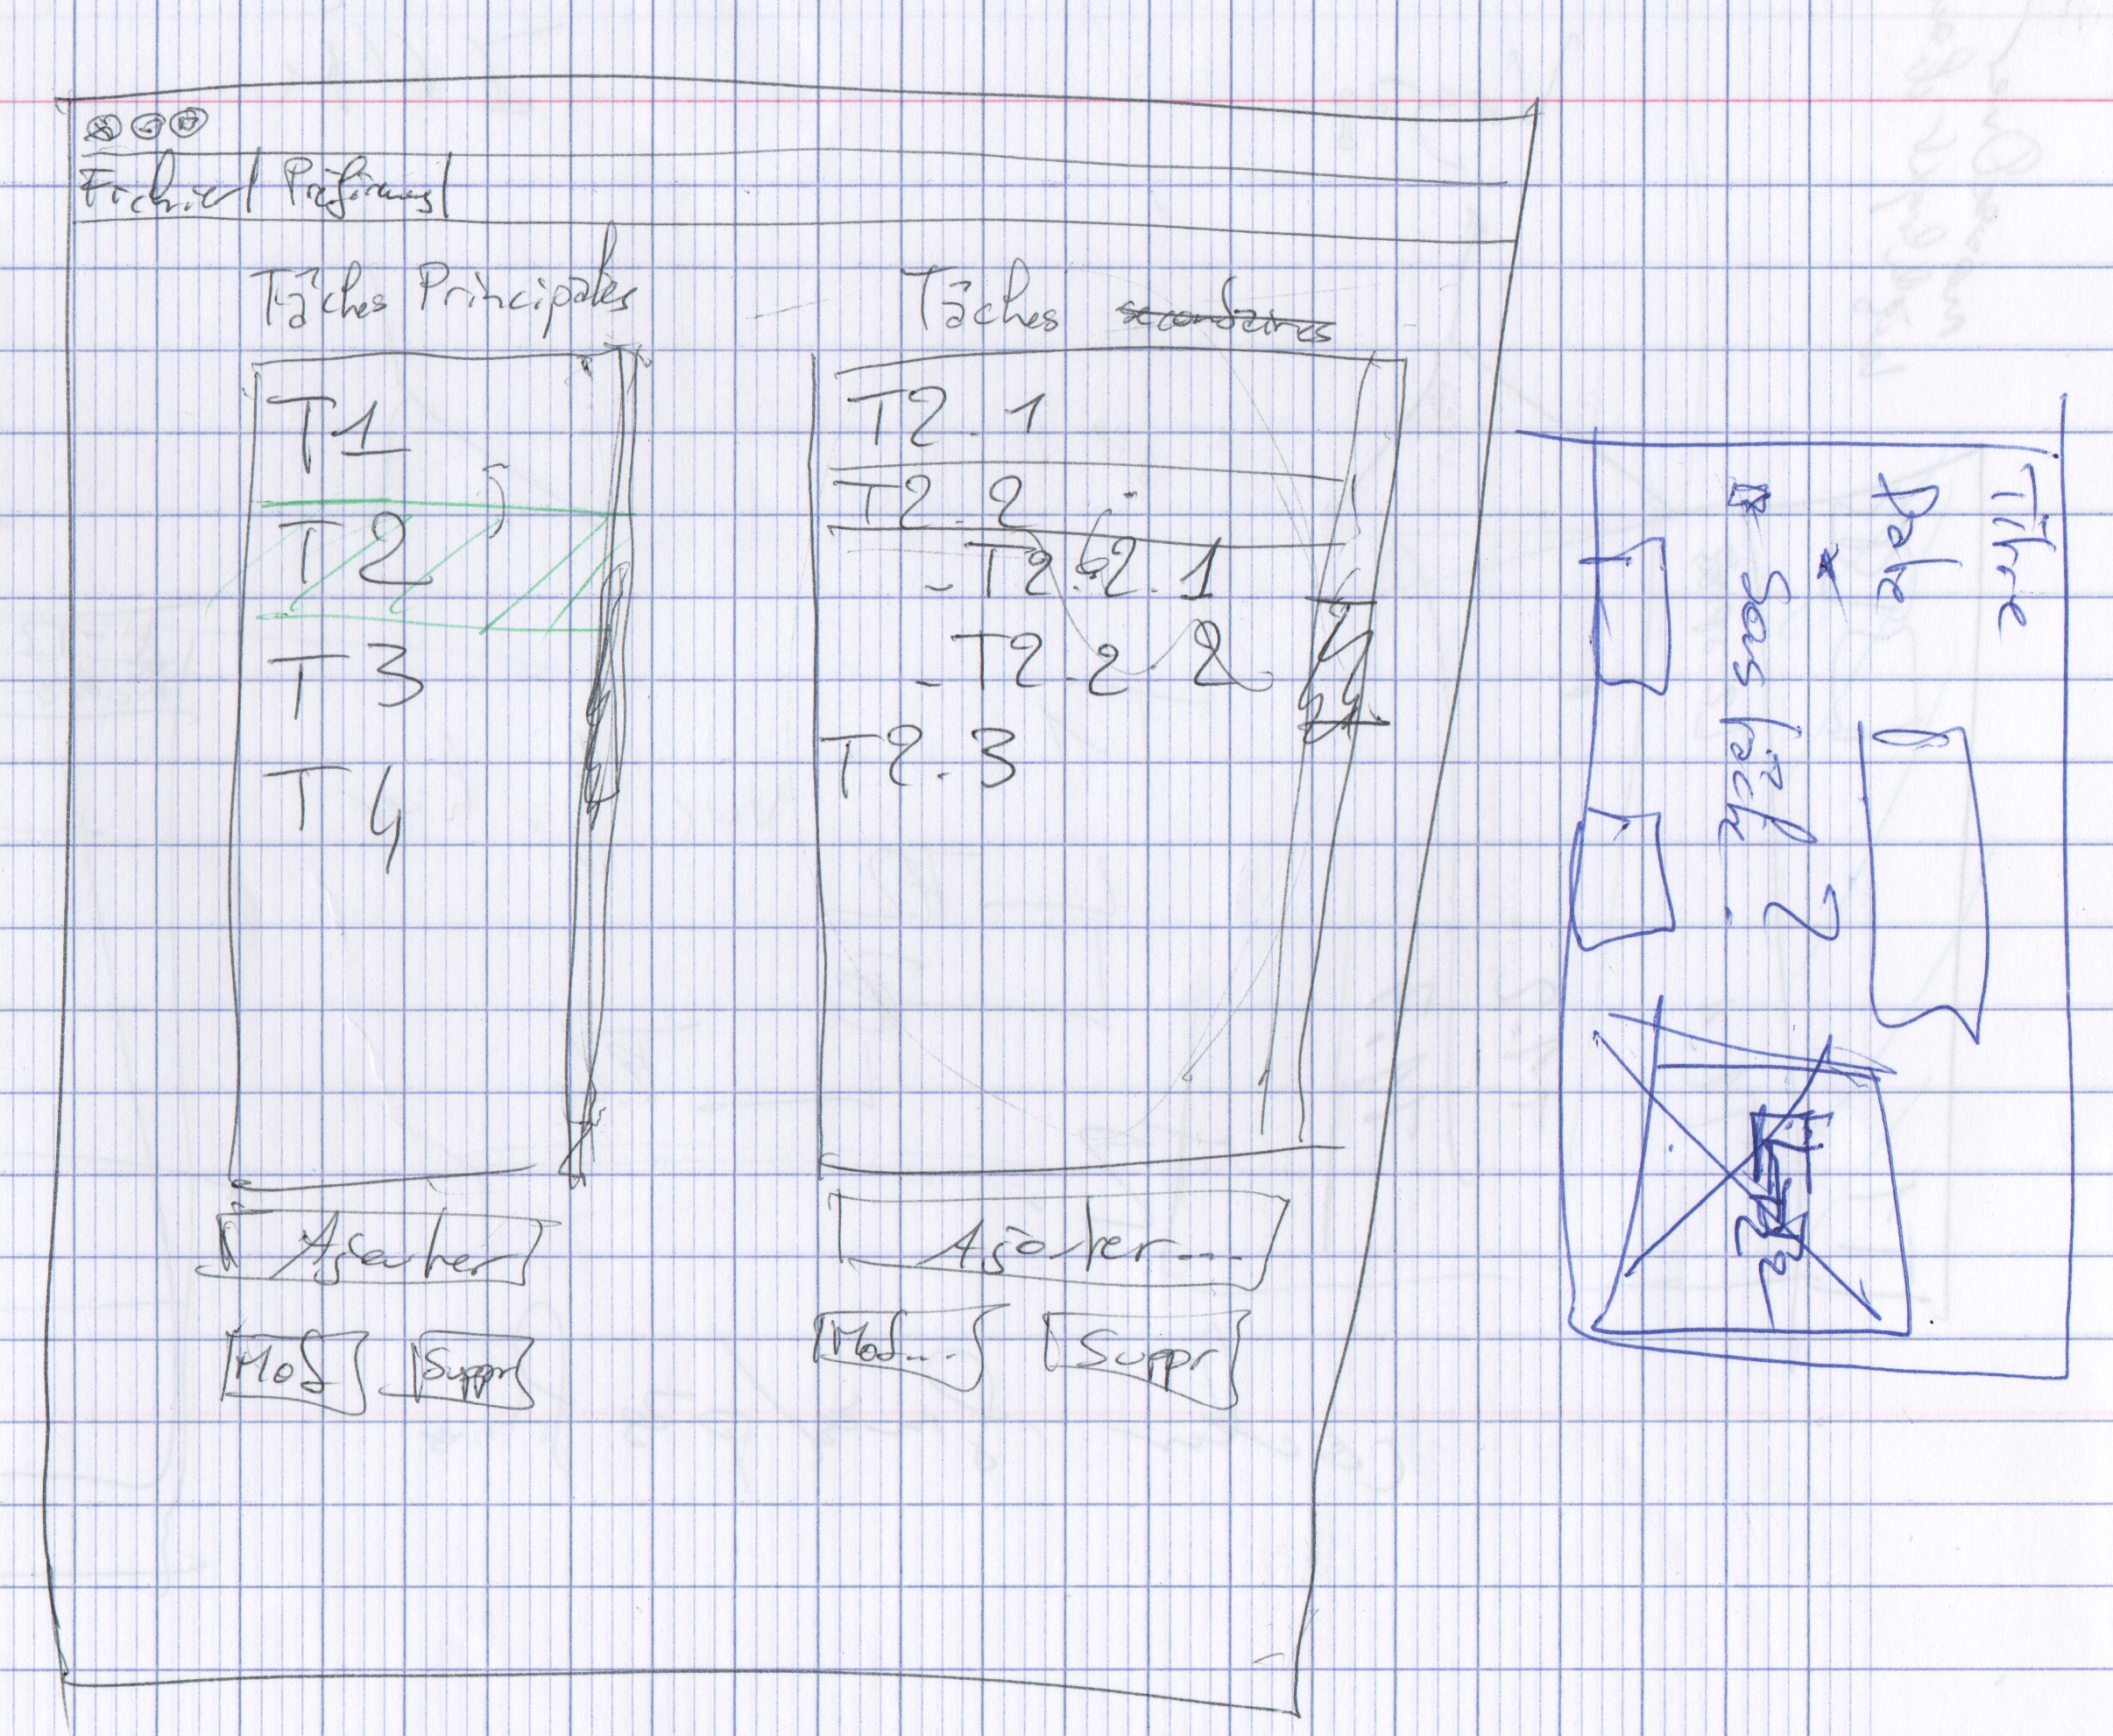
\includegraphics[width=12cm]{img/sobre.jpg}
  \caption{Working copy montrant l'interface sobre}
  \label{fig:sobre}
\end{figure}

\begin{figure}[H]
  \centering
  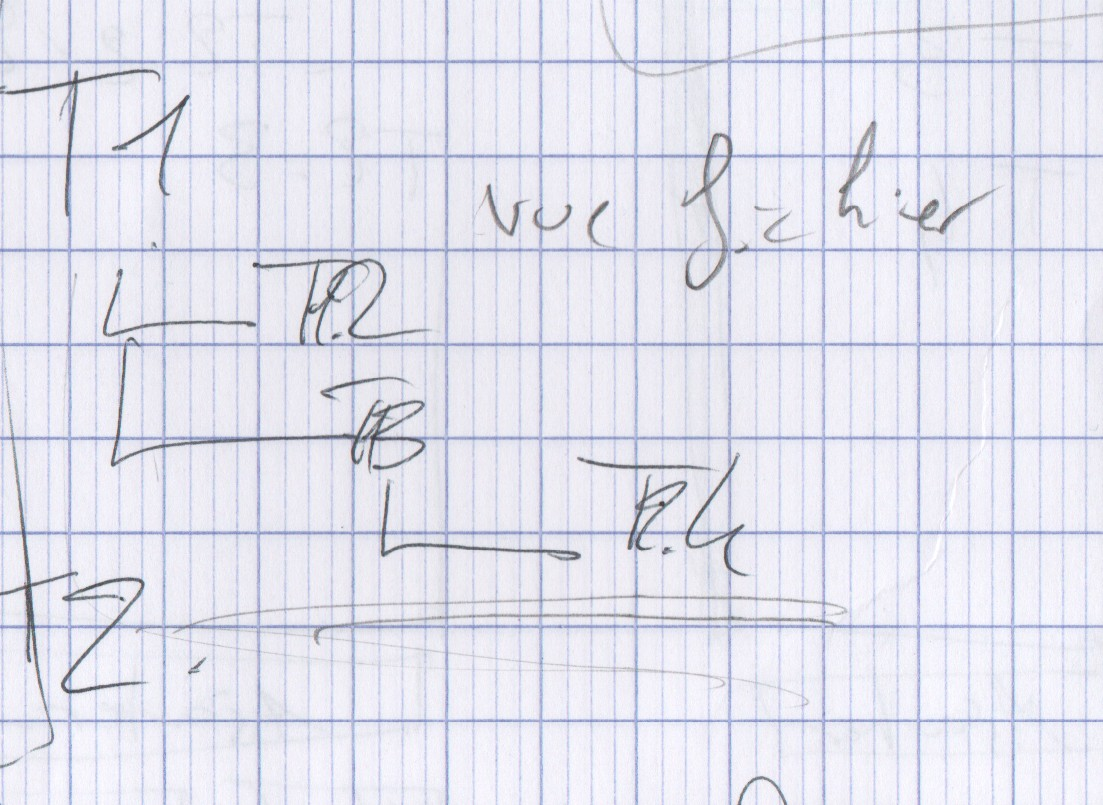
\includegraphics[width=12cm]{img/connue.jpg}
  \caption{Working copy montrant l'interface connue}
  \label{fig:connue}
\end{figure}

\begin{figure}[H]
  \centering
  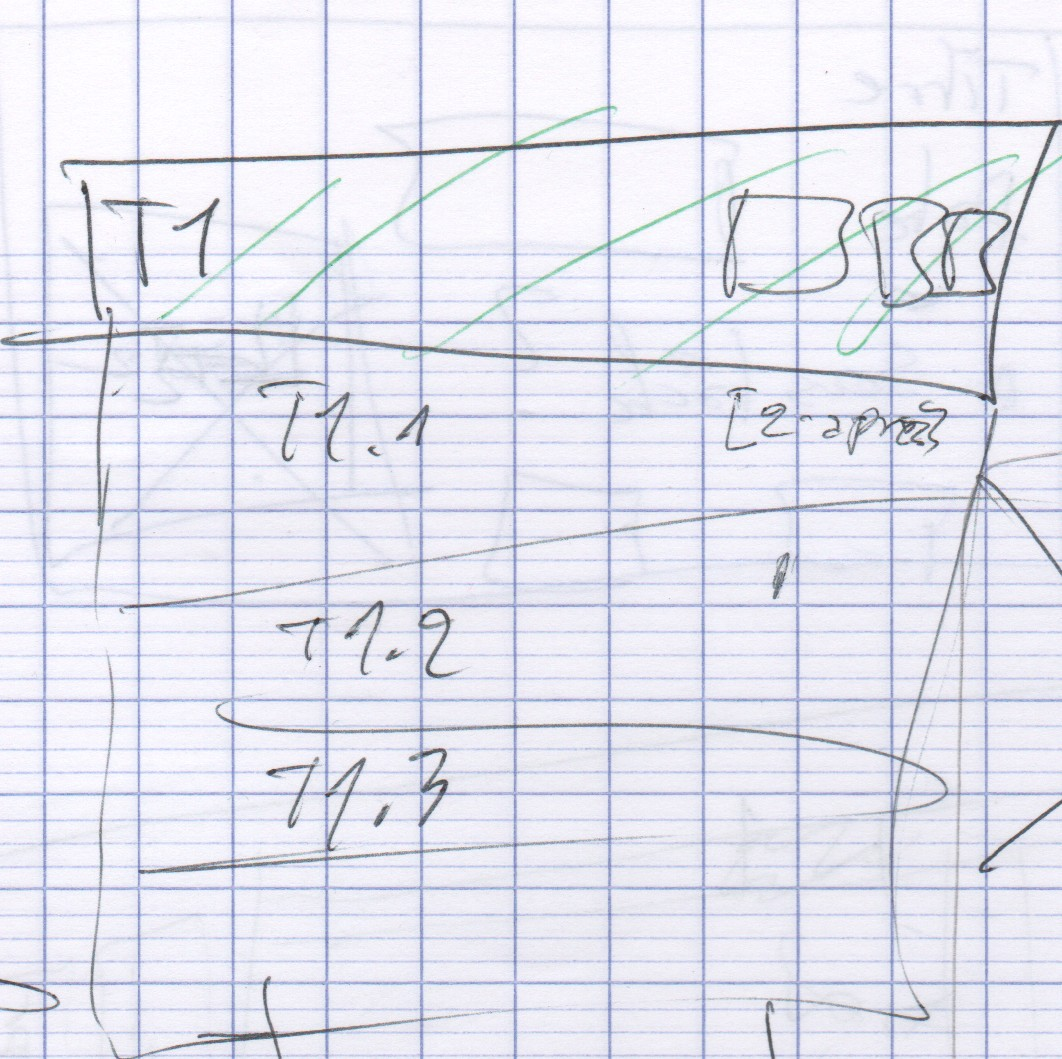
\includegraphics[width=12cm]{img/sexy.jpg}
  \caption{Working copy montrant l'interface sexy}
  \label{fig:sexy}
\end{figure}

C'est la troisième interface qui a été retenue.

\subsection{Trop de boutons +}
\label{ann:plusplusplus}

Nous avons voulu avoir une idée de l'interface en cas de forte
présences de boutons +.

\begin{figure}[H]
  \centering
  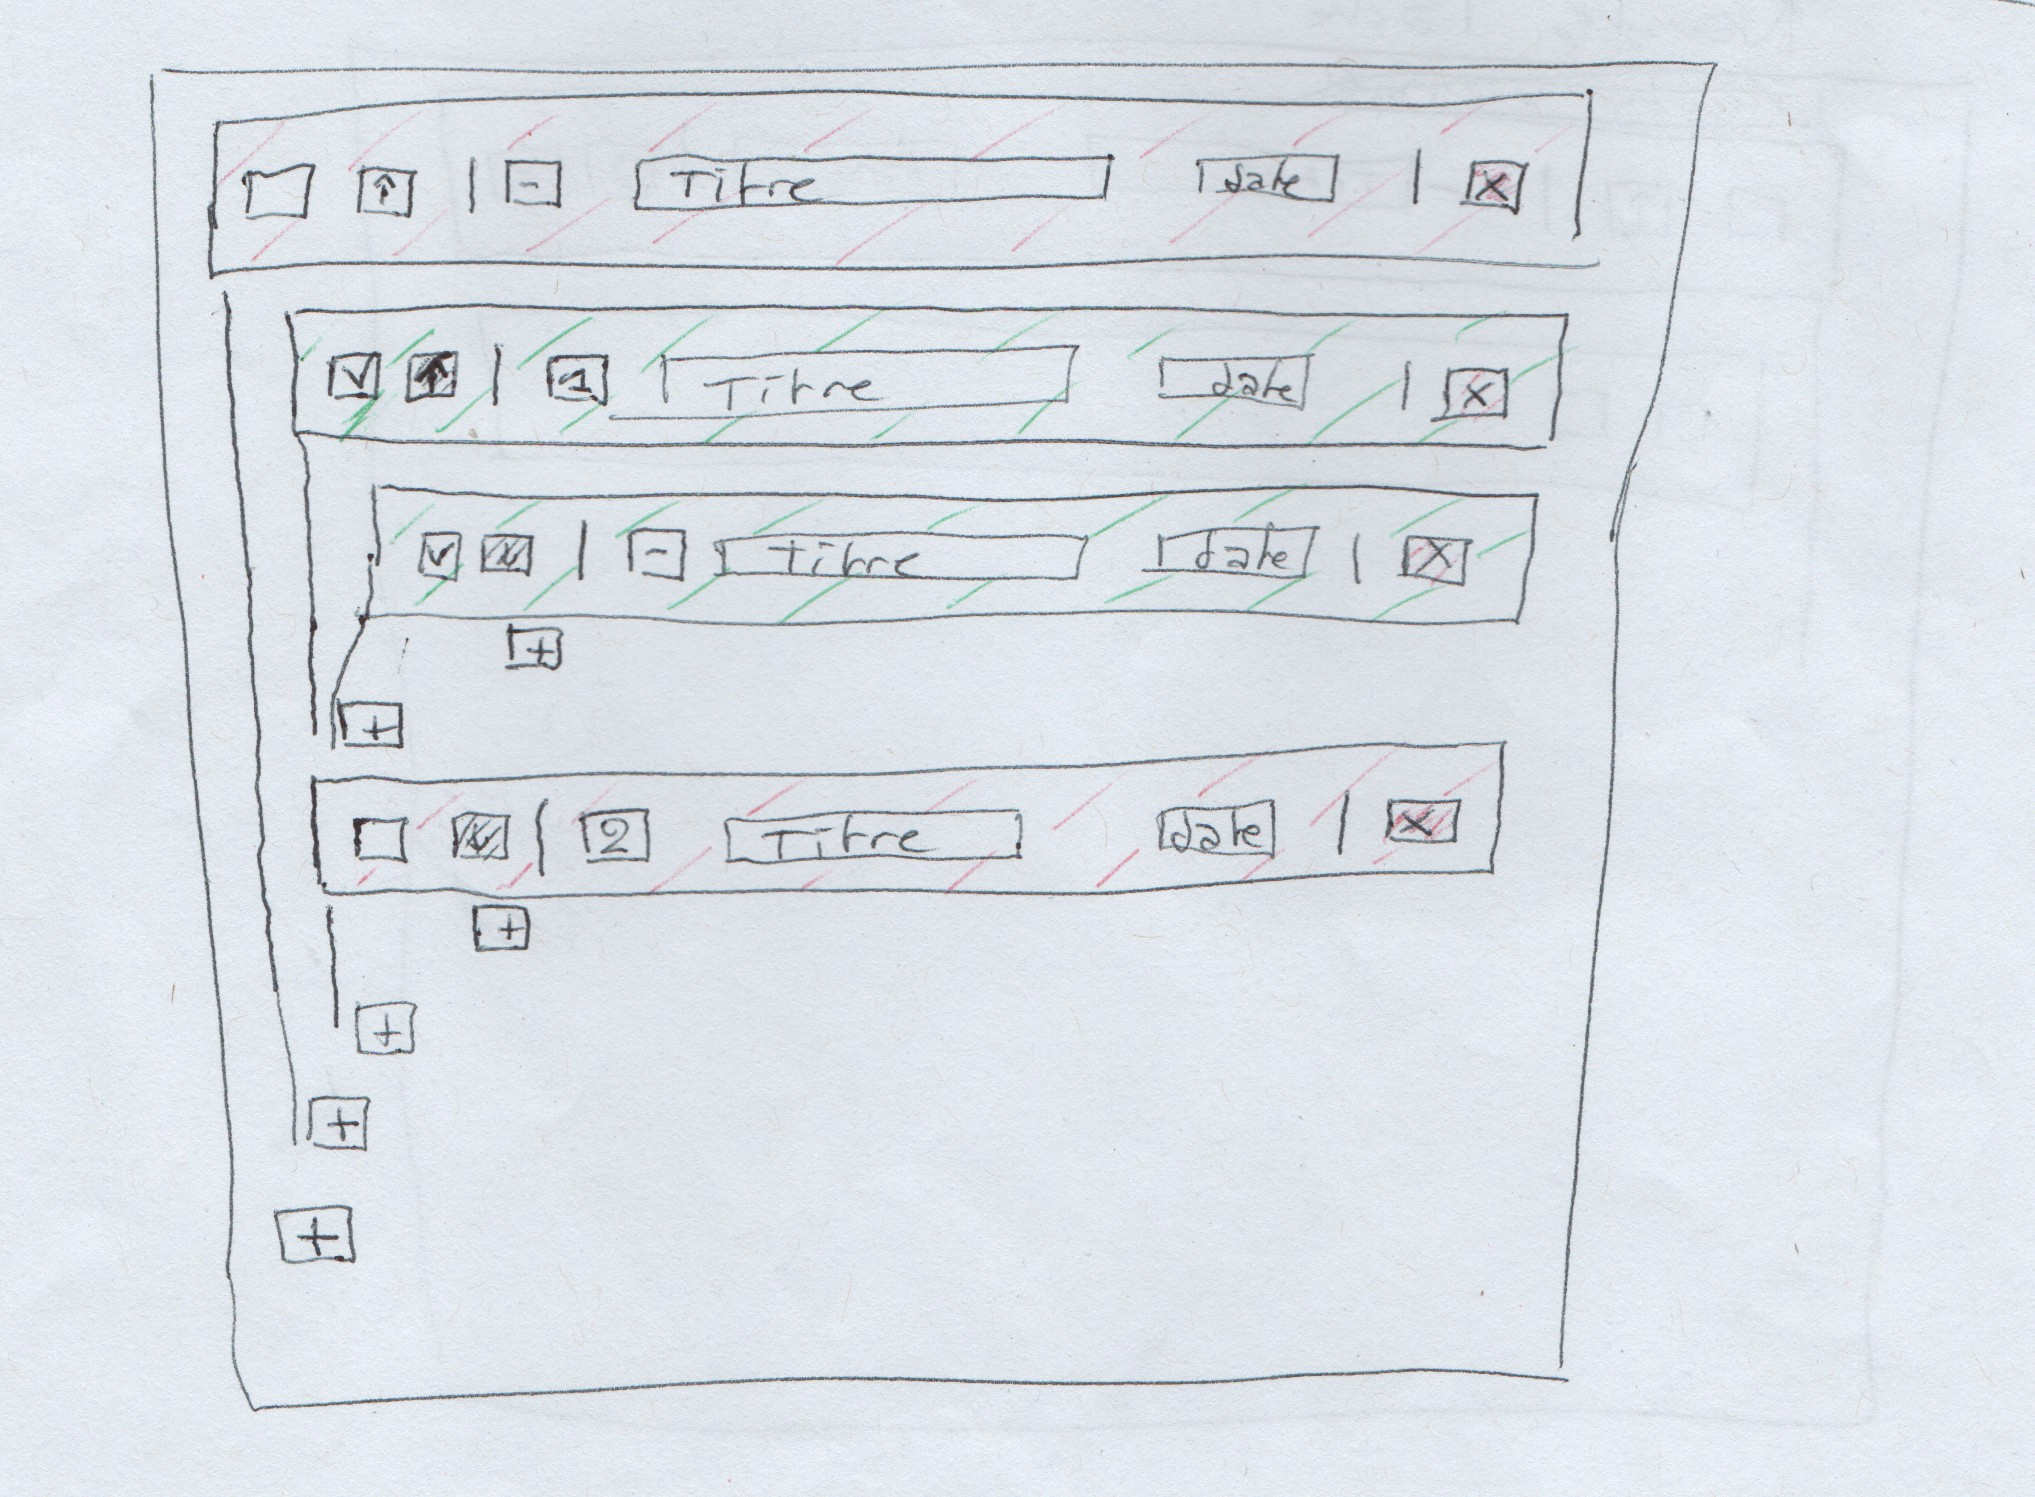
\includegraphics[width=12cm]{img/massboutons.jpg}
  \caption{Working copy montrant un grand nombre de boutons +}
  \label{fig:massplus}
\end{figure}

\subsection{Les votes}
\label{ann:votes}

Les working copies suivantes montrent les votes réalisés et les choix
proposés lors de ces votes.

\begin{figure}[H]
  \centering
  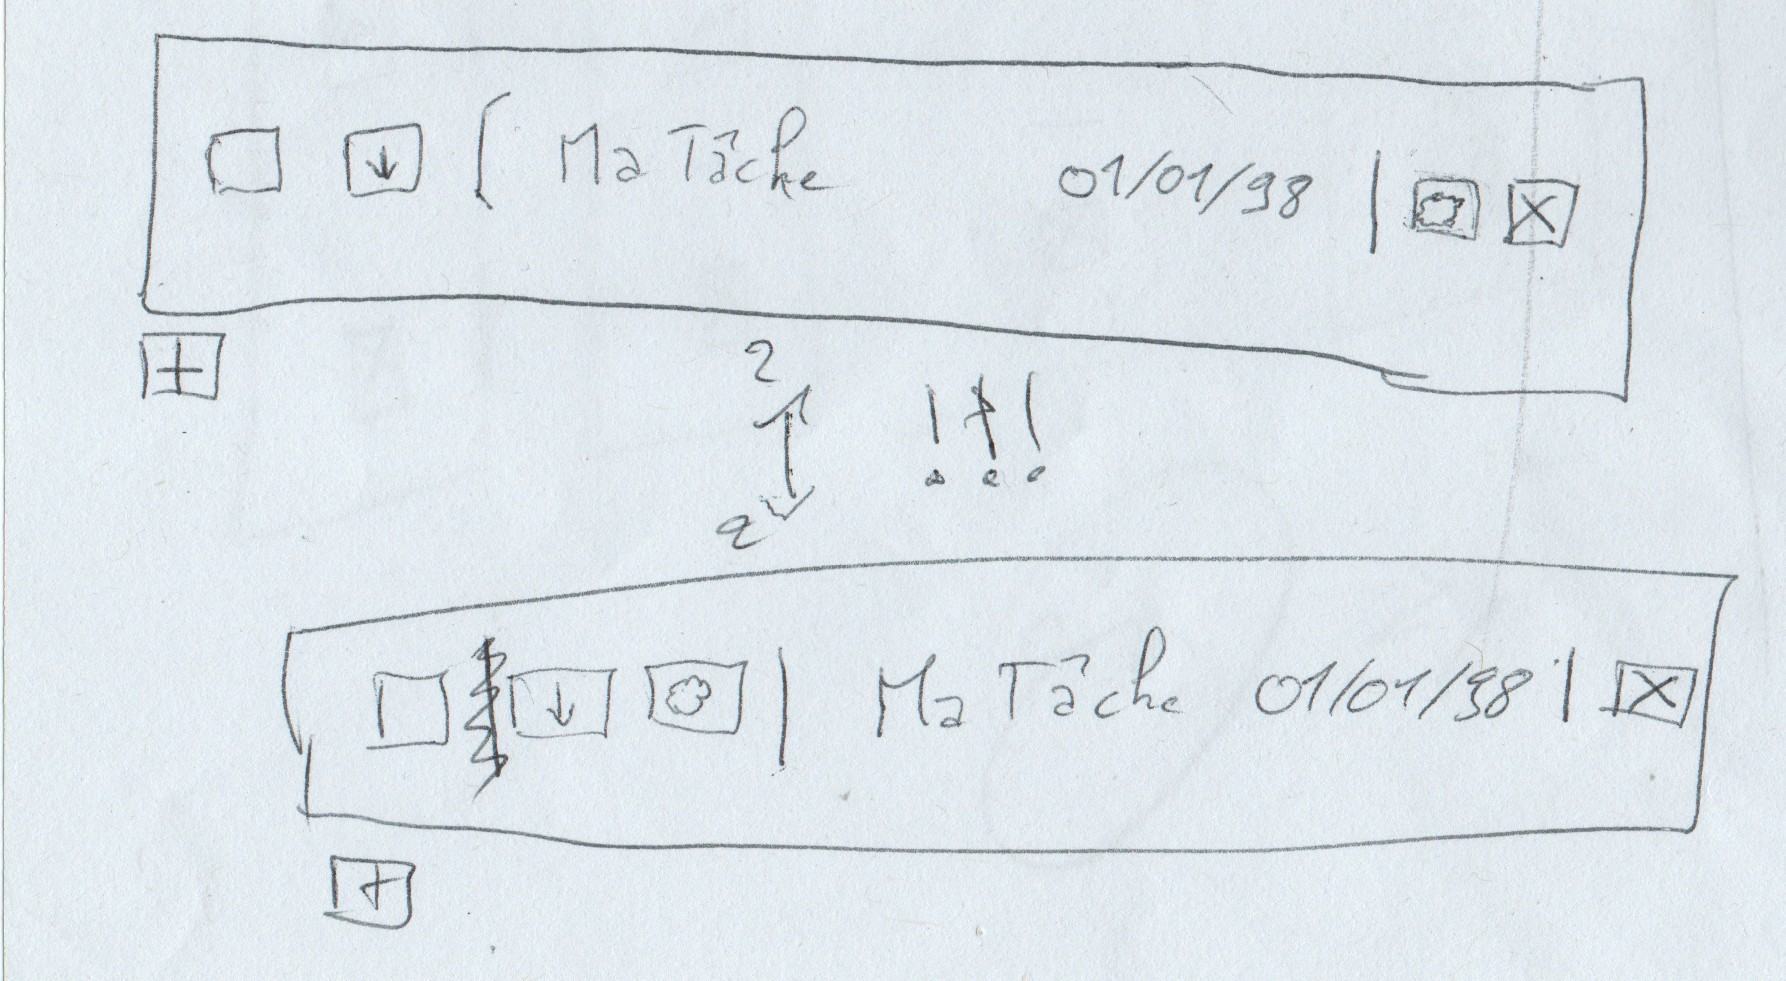
\includegraphics[width=12cm]{img/paramvote.jpg}
  \caption{Working copy montrant le vote pour le placement du bouton paramètres}
  \label{fig:paramvote}
\end{figure}

\begin{figure}[H]
  \centering
  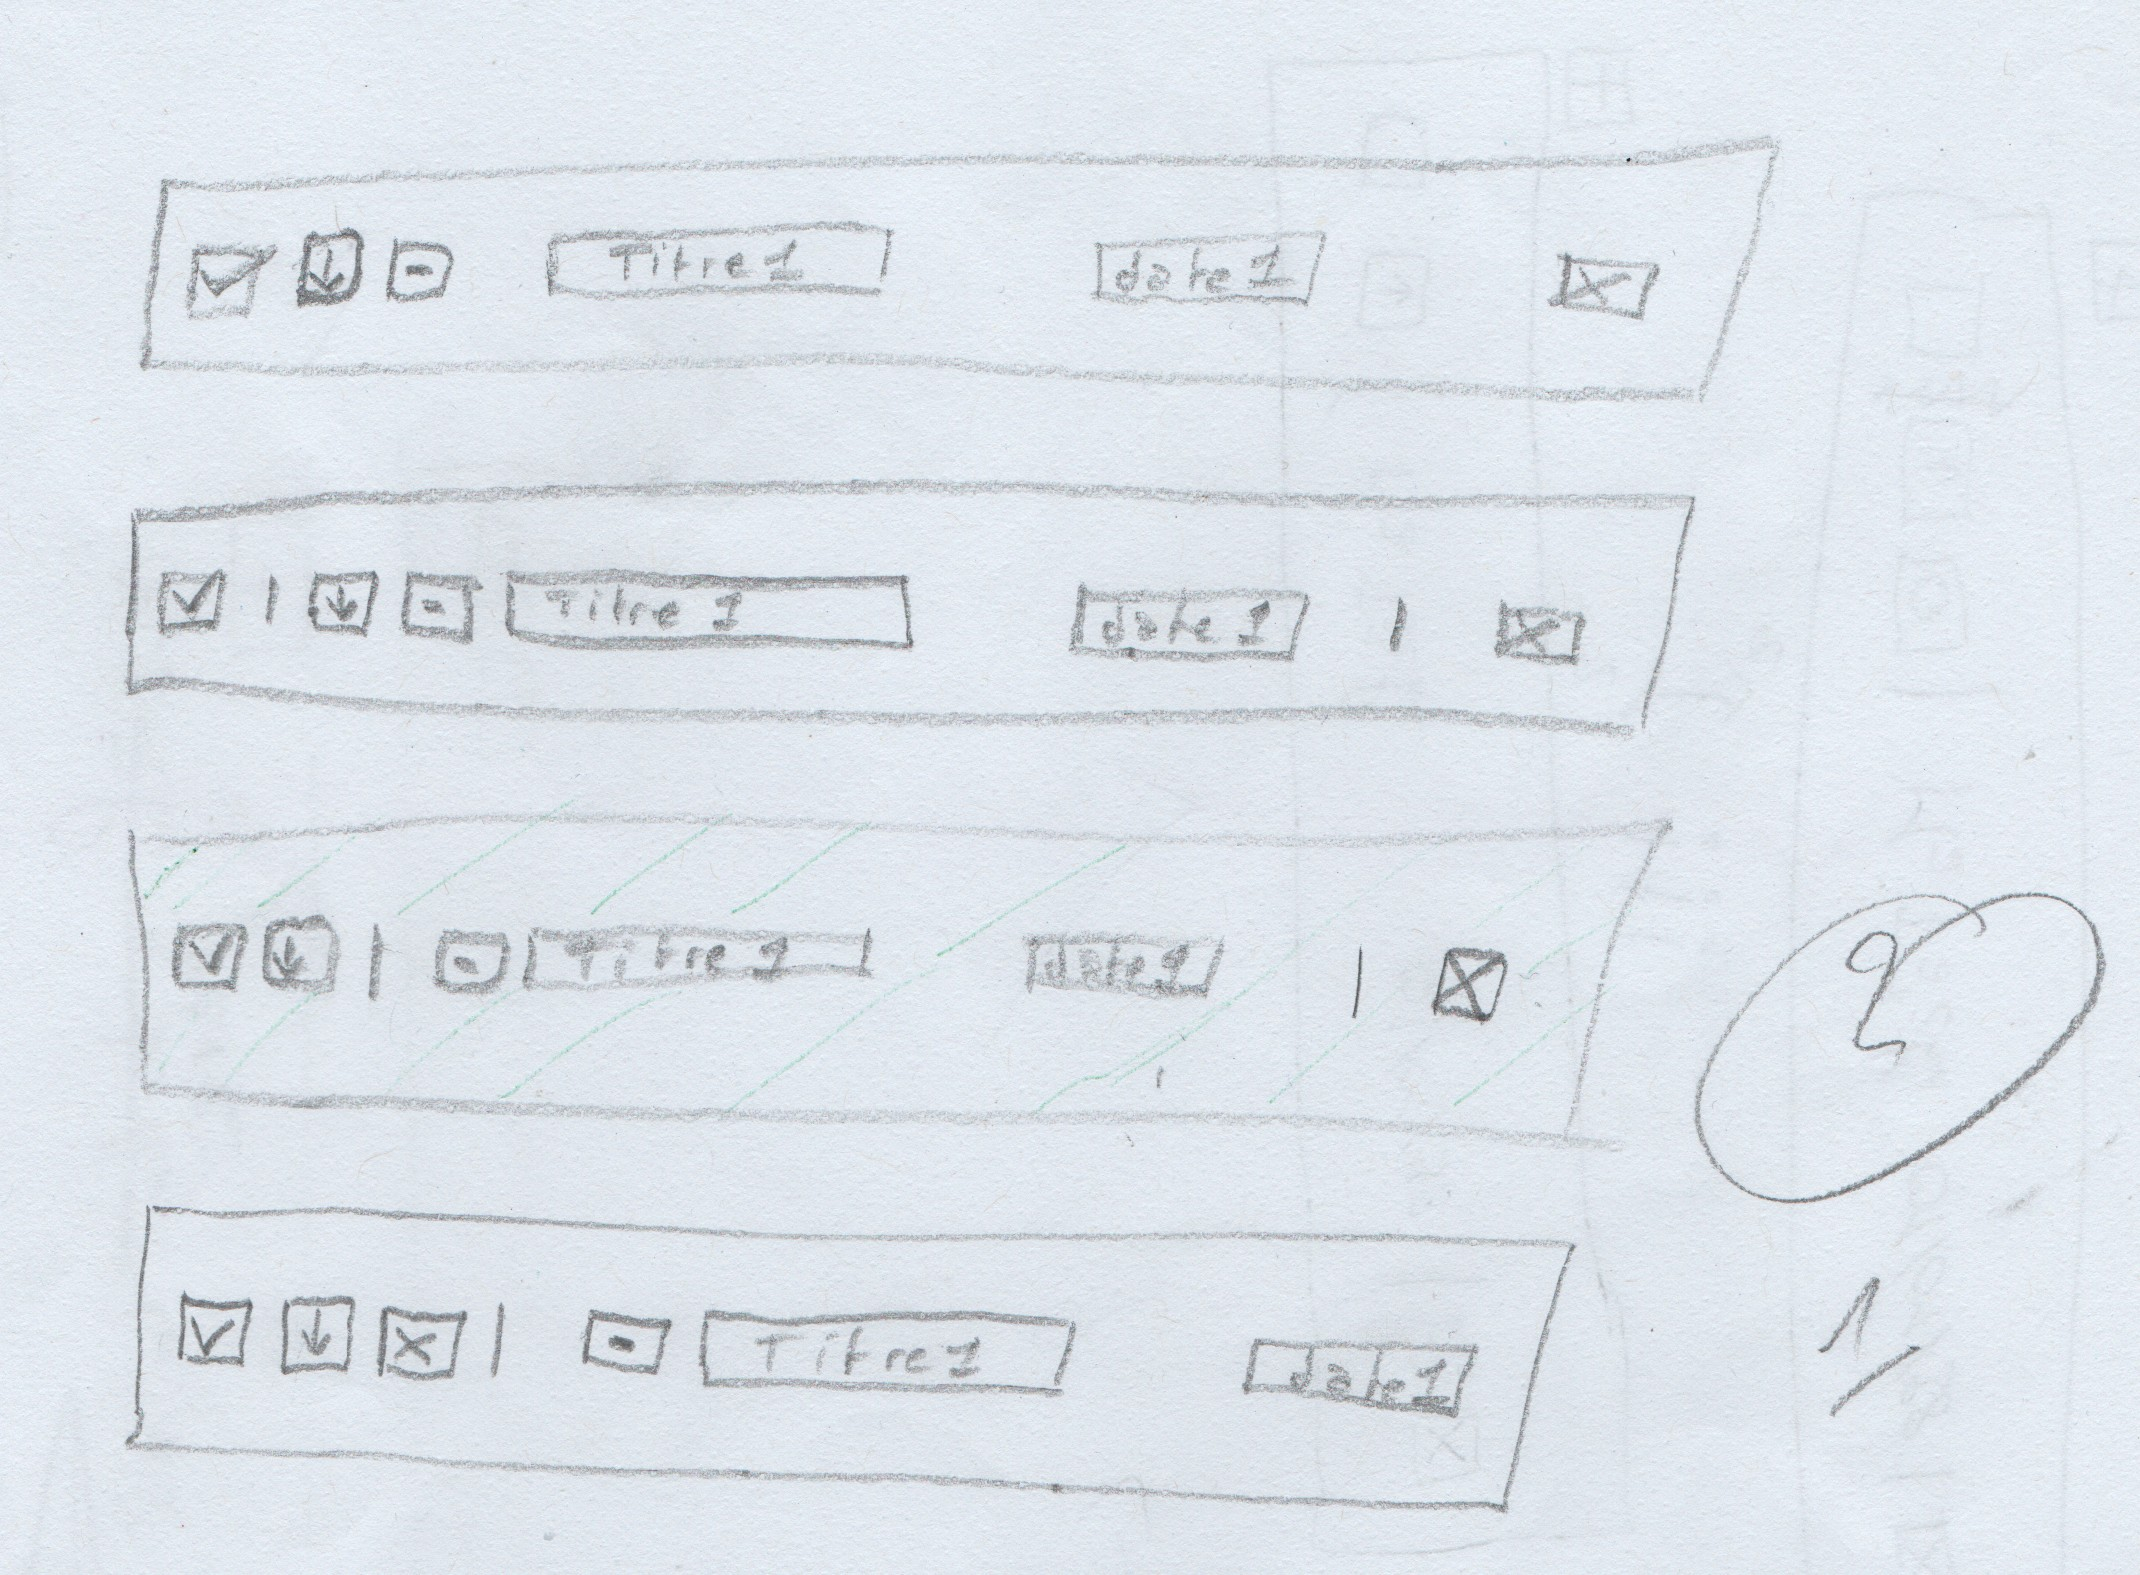
\includegraphics[width=12cm]{img/croixgroupevote.jpg}
  \caption{Working copy montrant le vote pour le placement de la croix
    et les groupes}
  \label{fig:croixgroupevote}
\end{figure}

\subsection{L'interface définitive}
\label{ann:interfacedef}

\begin{figure}[H]
  \centering
  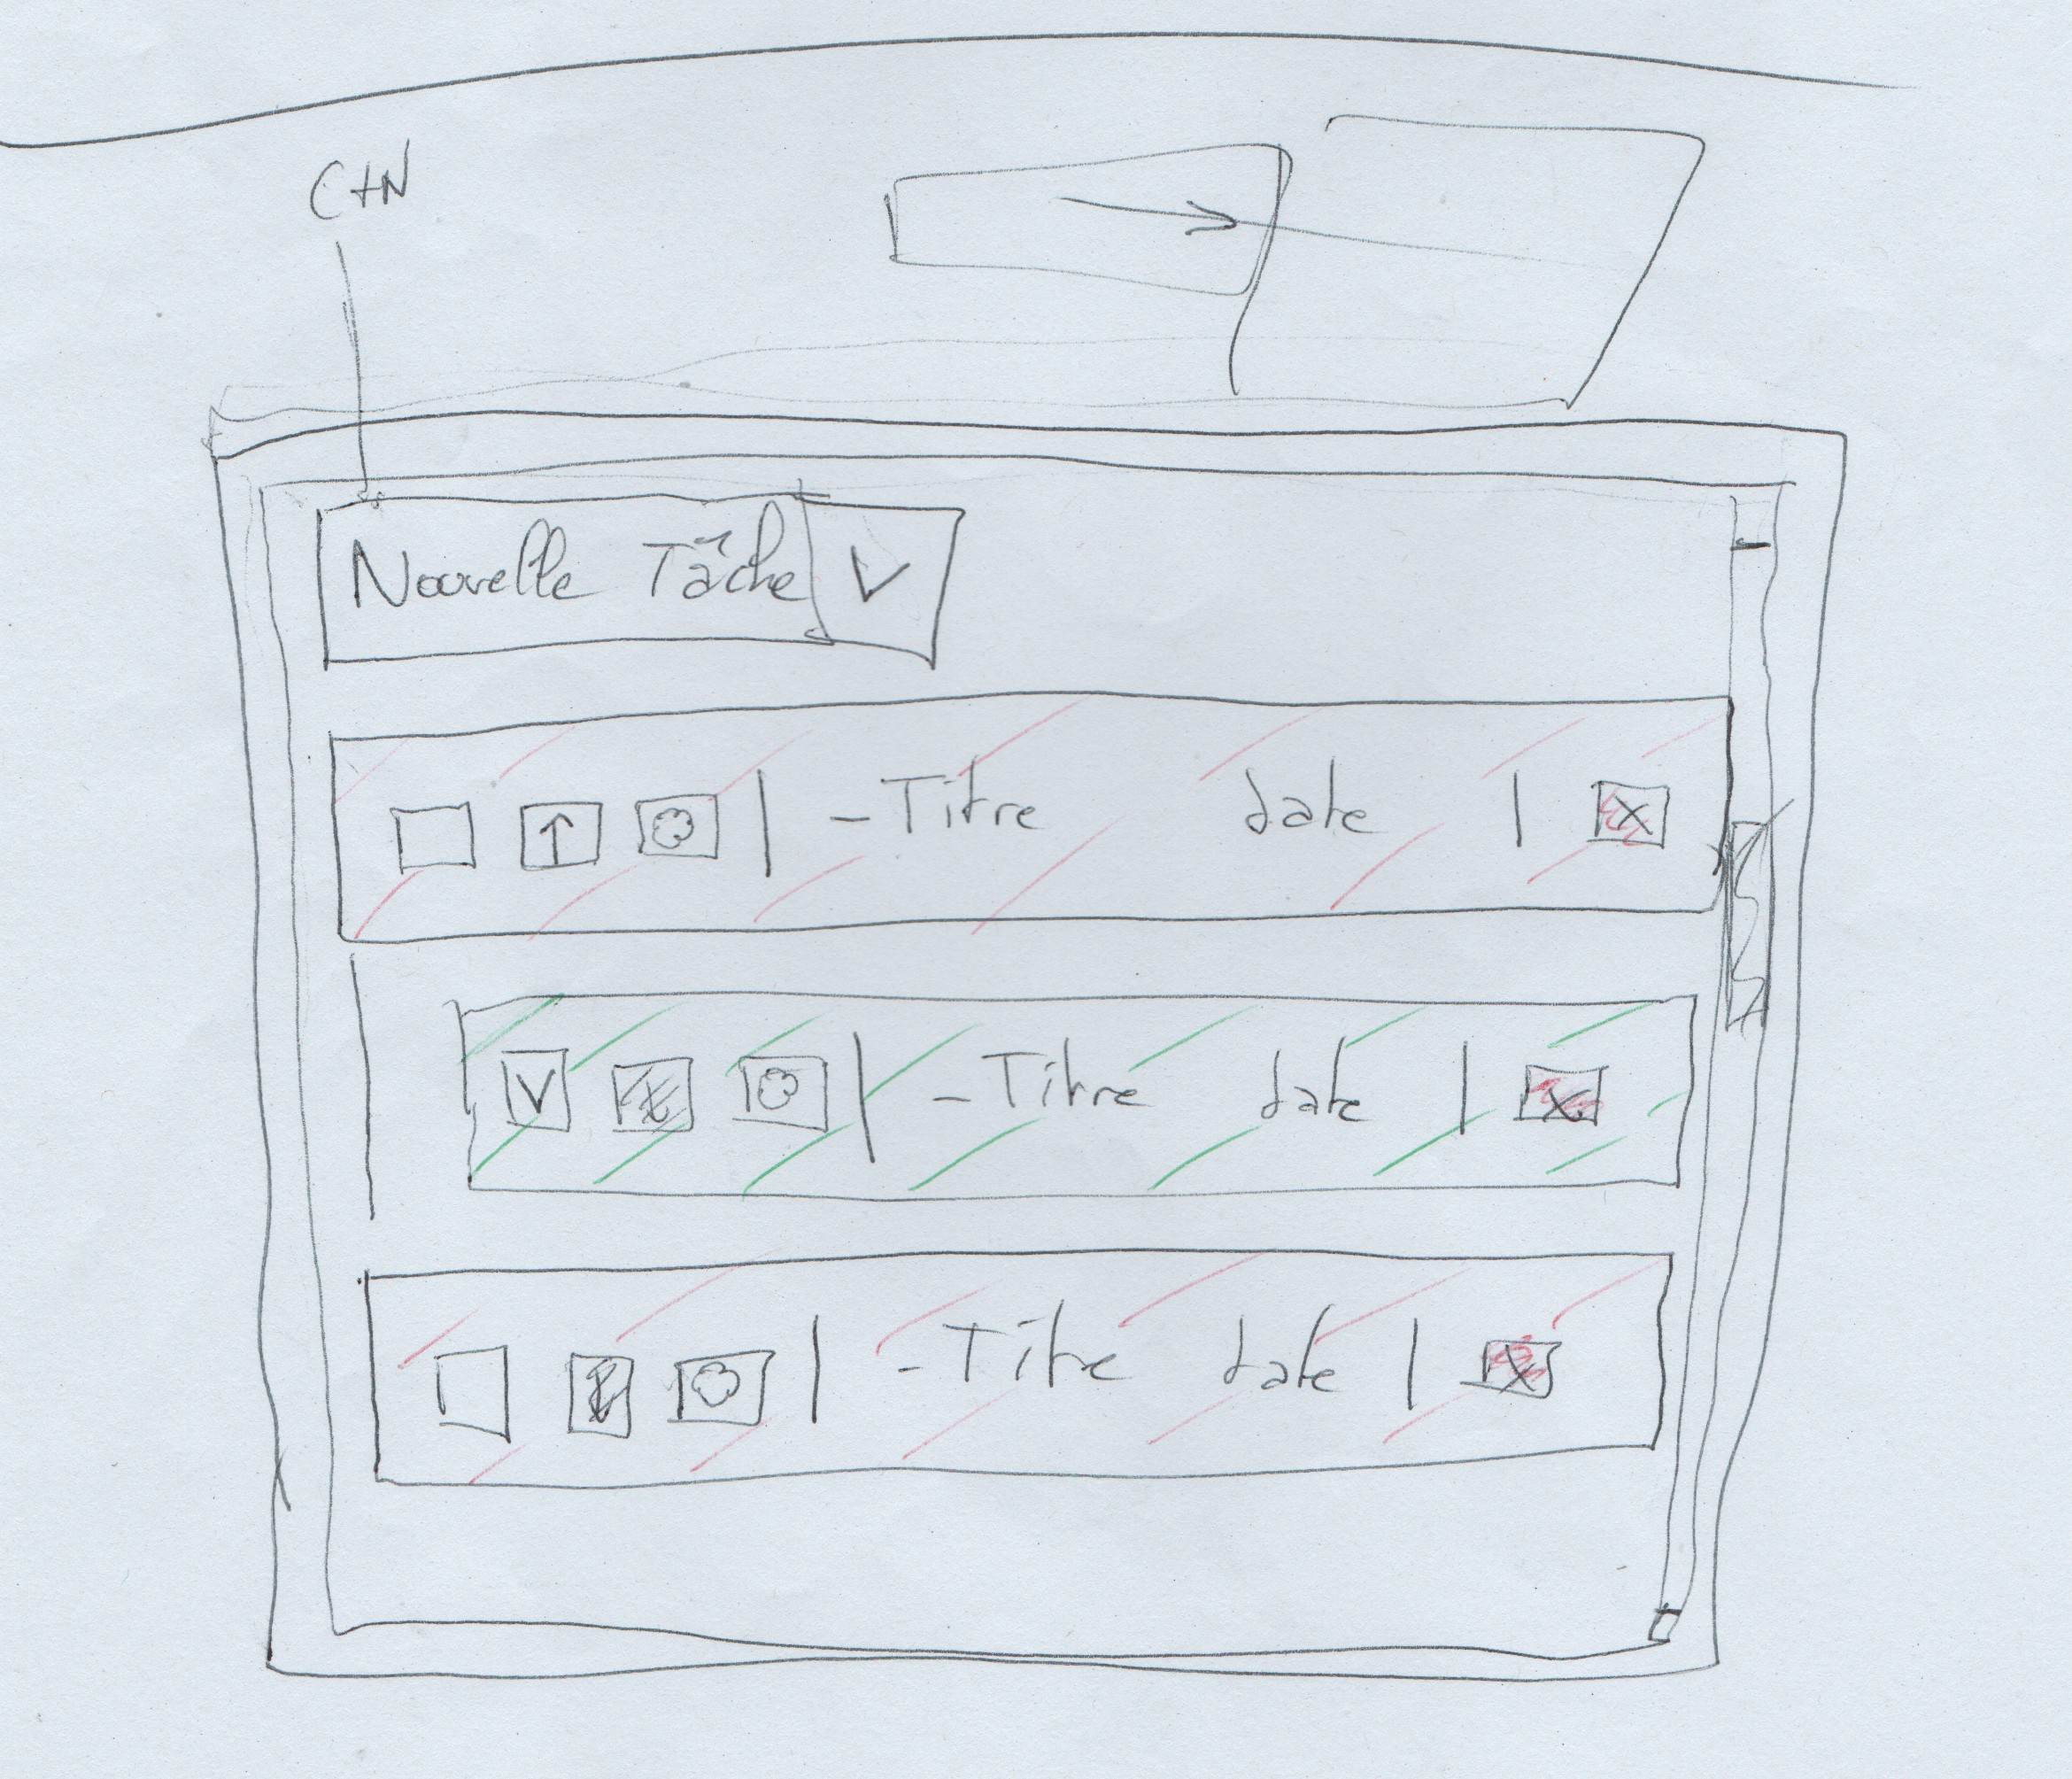
\includegraphics[width=12cm]{img/interfaceFinale.jpg}
  \caption{Working copy montrant l'interface finale attendue}
  \label{fig:interfacedefdessin}
\end{figure}

\begin{figure}[H]
  \centering
  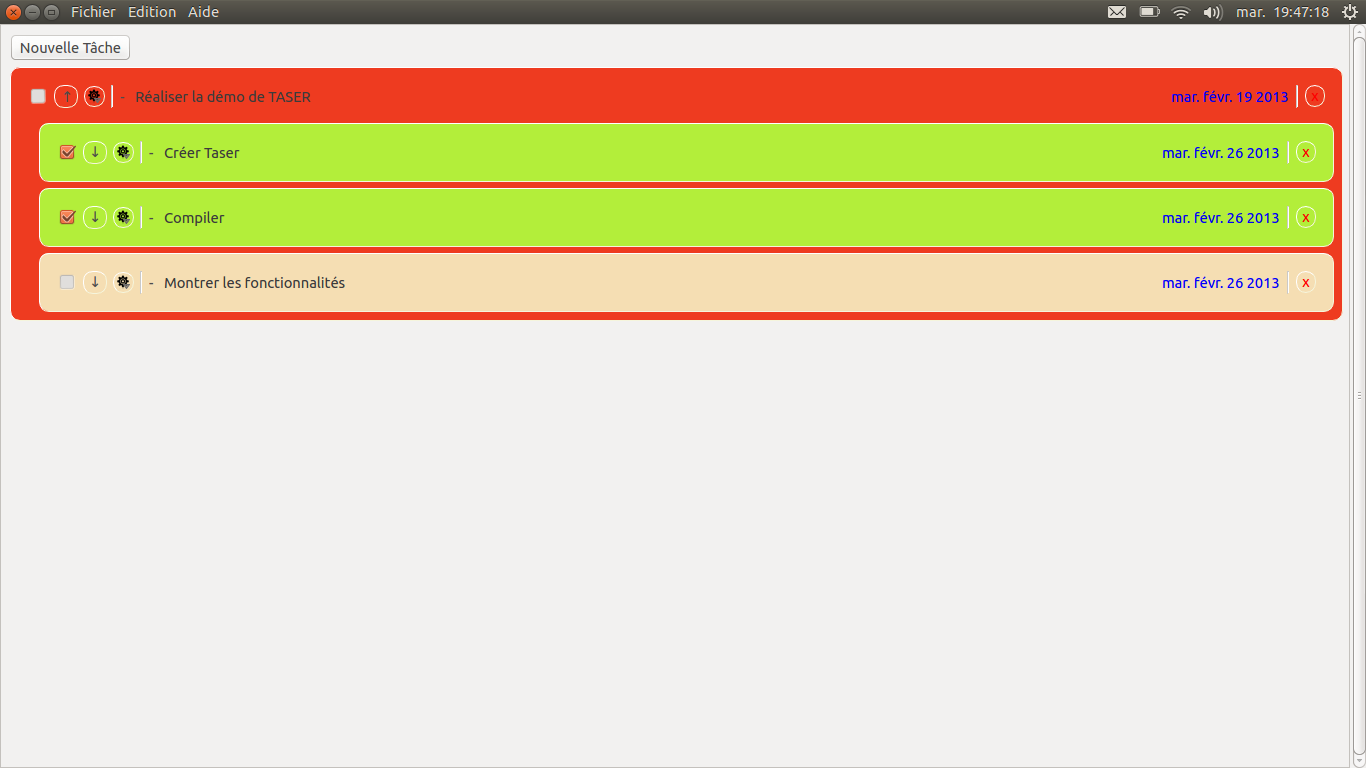
\includegraphics[width=12cm]{img/screen.png}
  \caption{Screenshot de l'application réalisée}
  \label{fig:interfacedefscreen}
\end{figure}


\end{document}
